\documentclass[11pt,a4paper]{article}

\usepackage[utf8]{inputenc}
\usepackage[T1]{fontenc}
\usepackage[brazil]{babel}
\usepackage{lmodern}
\usepackage{amsmath,amssymb,amsfonts,amsthm}
\usepackage{geometry}
\geometry{a4paper, left=18mm, right=18mm, top=22mm, bottom=22mm}
\usepackage{graphicx}
\usepackage{booktabs}
\usepackage{tabularx}
\usepackage{array}
\usepackage{xcolor}
\usepackage{microtype}
\usepackage{hyperref}
\usepackage{fancyhdr}
\usepackage{caption}
\usepackage{float}

\hypersetup{
    colorlinks=true,
    linkcolor=blue!80!black,
    citecolor=blue!80!black,
    urlcolor=blue!80!black,
    pdftitle={Entrega III - Descoberta e Validação Formal de Falhas Intrínsecas no Modelo Qwen 3.8 27B em Ambientes Virtuais Isolados - Mestrado PPGEE/UFAM},
    pdfauthor={Programa de Pós-Graduação em Engenharia Elétrica (PPGEE/UFAM)}
}

\pagestyle{fancy}
\fancyhf{}
\fancyhead[L]{\small\textcolor{gray}{Mestrado PPGEE/UFAM $\bullet$ Entrega III: Auditoria de Falhas Intrínsecas no Qwen 3.8 27B (Z3 SMT \& Ambientes Isolados)}}
\fancyhead[R]{\small\textcolor{gray}{\thepage}}
\fancyfoot[L]{\small\textcolor{gray}{Programa de Pós-Graduação em Engenharia Elétrica -- Universidade Federal do Amazonas}}
\fancyfoot[R]{\small\textcolor{gray}{Novembro de 2026}}
\renewcommand{\headrulewidth}{0.4pt}
\renewcommand{\footrulewidth}{0.4pt}

\theoremstyle{definition}
\newtheorem{definition}{Definição}
\newtheorem{theorem}{Teorema}
\newtheorem{lemma}{Lema}
\newtheorem{corollary}{Corolário}

\definecolor{ufamblue}{RGB}{15, 45, 105}

\begin{document}

\begin{titlepage}
    \centering
    \vspace*{0.3cm}
    {\Huge\bfseries\color{ufamblue} UNIVERSIDADE FEDERAL DO AMAZONAS \par}
    \vspace{0.25cm}
    {\Large\bfseries Faculdade de Tecnologia -- FT \par}
    {\large Programa de Pós-Graduação em Engenharia Elétrica -- PPGEE \par}
    {\normalsize Curso de Mestrado Acadêmico em Engenharia Elétrica \par}
    \vspace{0.85cm}
    
    \rule{\linewidth}{1.5pt} \\[0.35cm]
    {\large\bfseries ENTREGA CIENTÍFICA III -- AUDITORIA PROFUNDA DE VULNERABILIDADES INTRÍNSECAS \par}
    \vspace{0.25cm}
    {\LARGE\bfseries Descoberta e Validação Formal em Ambientes Virtuais Isolados de Falhas Estruturais, Numéricas (IEEE-754) e de \textit{Liveness} no Modelo Híbrido Qwen 3.8 27B \par}
    \rule{\linewidth}{1.5pt} \\[0.75cm]
    
    \begin{minipage}{0.98\textwidth}
        \small
        \begin{tabularx}{\linewidth}{l X}
            \textbf{Programa Acadêmico:} & Mestrado em Engenharia Elétrica (PPGEE -- FT/UFAM) \\
            \textbf{Linha de Pesquisa:} & Métodos Formais, Verificação Simbólica (ESBMC/Z3 SMT) e Auditoria de Modelos de Linguagem \\
            \textbf{Padrão de Qualidade:} & Estrutura Científica Canônica (IMRaD) com Rigor de Nível Internacional (\textit{CAV / TACAS / IEEE TSE}) \\
            \textbf{Objeto de Auditoria:} & \textbf{Qwen 3.8 27B (\texttt{qwen3.8:27b}):} Arquitetura híbrida \texttt{qwen35} ($27.320.697.856$ parâmetros, 65 blocos: 48 Gated-DeltaNet/Mamba-2 SSM + 16 Full Attention com QK-Norm + 1 bloco Multi-Token Prediction \texttt{nextn}, 863 tensores, binário GGUF de $16{,}81\text{ GB}$) \\
            \textbf{Ambientes Virtuais de Prova:} & \textbf{1. Venv Remoto de Extração e Prova:} \texttt{venv\_flaw\_audit} (Python 3.14 isolado + Z3 SMT 4.13) \\
            & \textbf{2. Venv Local de Dupla Confirmação:} \texttt{venv\_local\_flaw\_check} (Python 3.12 isolado + Z3 \texttt{QF\_FP}/\texttt{QF\_NRA}) \\
            \textbf{Infraestrutura Computacional:} & Servidor HPC Dedicado: GPU NVIDIA RTX 2000 Ada (16 GB) + Intel Core i7-14700 (28 Threads) \\
            \textbf{Data:} & Novembro de 2026
        \end{tabularx}
    \end{minipage}
    
    \vspace{0.6cm}
    \begin{minipage}{0.98\textwidth}
        \footnotesize
        \begin{center}\textbf{RESUMO}\end{center}
        \noindent Embora a varredura macroscópica de integridade do modelo \textbf{Qwen 3.8 27B (\texttt{qwen3.8:27b})} confirme a ausência de valores inválidos estáticos (\texttt{0 NaN / 0 Inf} nos 863 tensores), uma auditoria microscópica bit-a-bit guiada por verificação formal SMT nas lógicas \texttt{QF\_FP} (IEEE-754 \texttt{binary32}), \texttt{QF\_NRA} (Aritmética Real Não-Linear) e \texttt{QF\_LIA} revelou \textbf{quatro falhas intrínsecas reais e inéditas} alojadas diretamente nos pesos e metadados do modelo. Para assegurar reprodutibilidade científica estrita e ausência de contaminação de estado, todas as provas foram executadas e duplamente confirmadas em dois \textbf{ambientes virtuais Python isolados e independentes} (\texttt{venv\_flaw\_audit} no servidor HPC e \texttt{venv\_local\_flaw\_check} na estação de verificação). As quatro falhas descobertas e provadas formalmente (\texttt{SAT} com geração de contraexemplos exatos no Z3) são: \textbf{(i) Falha 1 (\texttt{FLAW-01}): Colapso de Posto (\textit{Rank Collapse}) e Envenenamento de Denominador RMS por Pesos Exatamente Zero (\texttt{0x00000000})} nos tensores \texttt{blk.7.post\_attention\_norm.weight[3994]}, \texttt{blk.43.attn\_k\_norm.weight[32]} e \texttt{blk.59.attn\_q\_norm.weight[1]}, permitindo que perturbações no subespaço nulo suprimam em até \textbf{96,81\%} o ganho dos 255 canais ativos; \textbf{(ii) Falha 2 (\texttt{FLAW-02}): Inversão Antipodal de Fase ($180^\circ$) no \texttt{QK-Norm} sobre Planos Primários RoPE} em \texttt{blk.31.attn\_k\_norm[0]} ($-0{,}1484375$), \texttt{blk.47.attn\_k\_norm[0]} ($-0{,}0390625$) e \texttt{blk.59.attn\_k\_norm[32]} ($-0{,}0078125$), quebrando a monotonicidade de autossimilaridade cosseno ($\Delta pos = 0$); \textbf{(iii) Falha 3 (\texttt{FLAW-03}): Violação do Horizonte Exponencial IEEE-754 \texttt{float32} ($|a| > 88{,}722839$) e Regime Subnormal/Underflow} no bloco recorrente \texttt{blk.12.ssm\_a} (Cabeça 41 com $a = -139{,}4213$, \texttt{0xC30B6BD8}, causando \textit{underflow} total $\exp(a) = \texttt{0x00000000}$ e perda de $99{,}81\%$ de memória por passo; e Cabeça 9 com $a = -102{,}0028$, \texttt{0xC2CC016C}, cujo $\exp(a) = \texttt{0x00000004}$ cai no regime subnormal/denormal IEEE-754 com perda de 21 dos 24 bits de mantissa); e \textbf{(iv) Falha 4 (\texttt{FLAW-04}): Violação Determinística de \textit{Liveness} (\textit{Output Starvation})} no template de chat embutido no GGUF (\texttt{reasoning\_effort = 'xhigh'} por padrão), que consome $100\%$ do orçamento sob limites de predição moderados e retorna saída visível vazia (\texttt{response = ""}).
    \end{minipage}
    
    \vfill
    {\small Manaus -- Amazonas, Brasil $\bullet$ 2026 \par}
\end{titlepage}

\newpage
\tableofcontents
\vspace{0.4cm}
\hrule
\vspace{0.4cm}

% =============================================================================
\section{Introdução}
% =============================================================================

A certificação formal de Grandes Modelos de Linguagem (\textit{Large Language Models} -- LLMs) exige distinguir dois níveis complementares de verificação: (1) a \textbf{estabilidade macroscópica de propagação e robustez de fronteira de decisão}, na qual provamos que o vocabulário de saída permanece invariante sob perturbações limitadas $\|\delta\|_\infty \le \epsilon$; e (2) a \textbf{auditoria microscópica de patologias algébricas e numéricas intrínsecas aos tensores treinados}. Mesmo quando um modelo de 27,32 bilhões de parâmetros não apresenta valores estáticos inválidos (\texttt{NaN} ou \texttt{Inf}) armazenados diretamente em disco, anomalias sutis introduzidas durante o treinamento estocástico em precisão mista (\texttt{BF16}/\texttt{FP32}) ou durante a quantização pós-treinamento (\texttt{Q4\_K\_M}) podem criar singularidades locais no Jacobiano da rede, violações de invariantes geométricos nos subespaços de atenção e regimes de \textit{overflow}/\textit{underflow}/subnormalidade IEEE-754 em operadores exponenciais.

Neste terceiro relatório da série científica desenvolvida no \textbf{Mestrado em Engenharia Elétrica (PPGEE/UFAM)}, respondemos a uma questão investigativa central:
\begin{quote}
\textit{Existem falhas estruturais, algébricas, numéricas (IEEE-754) ou de vivacidade (liveness) intrínsecas ao próprio modelo \textbf{Qwen 3.8 27B (\texttt{qwen3.8:27b})}, e é possível provar formalmente a existência dessas vulnerabilidades mediante solucionadores SMT em ambientes virtuais estritamente isolados?}
\end{quote}

Através de uma varredura exaustiva dos 863 tensores e dos metadados estruturais do arquivo GGUF de $16{,}81\text{ GB}$ do \texttt{qwen3.8:27b}, combinada com formulações formais nas teorias \texttt{QF\_FP} (\textit{Quantifier-Free Floating-Point Arithmetic}, padrão IEEE-754 \texttt{binary32}), \texttt{QF\_NRA} (\textit{Quantifier-Free Nonlinear Real Arithmetic}) e \texttt{QF\_LIA} (\textit{Quantifier-Free Linear Integer Arithmetic}), identificamos e provamos formalmente (\texttt{SAT}) \textbf{quatro classes de falhas intrínsecas reais} no modelo Qwen 3.8 27B.

% =============================================================================
\section{Fundamentação Teórica das Invariantes Violadas}
% =============================================================================

Para formalizar rigorosamente cada falha encontrada no \texttt{qwen3.8:27b}, estabelecemos as definições e invariantes matemáticos que todo modelo híbrido Transformer/State-Space bem-condicionado deve satisfazer.

\subsection{Invariante de Posto Completo e Condicionamento do Operador \texttt{RMSNorm}}

Em cada bloco do Qwen 3.8 27B, o operador \textit{Root Mean Square Layer Normalization} ($\text{RMSNorm}_\gamma: \mathbb{R}^d \to \mathbb{R}^d$), parametrizado pelo vetor de escala $\gamma = (\gamma_0, \dots, \gamma_{d-1})^\top \in \mathbb{R}^d$ e constante de regularização $\varepsilon = 10^{-6}$, é definido por:
\begin{equation}
    y_i = \text{RMSNorm}_\gamma(z)_i = \frac{\gamma_i \cdot z_i}{\text{RMS}(z)}, \qquad \text{onde} \quad \text{RMS}(z) = \sqrt{\frac{1}{d}\sum_{j=0}^{d-1} z_j^2 + \varepsilon}.
    \label{eq:rmsnorm_def}
\end{equation}

\begin{definition}[Invariante de Não-Degenerescência Multiplicativa de \texttt{RMSNorm}]
Diz-se que uma camada $\text{RMSNorm}_\gamma$ preserva posto local e acoplamento energético consistente se, e somente se, todos os seus pesos de escala são estritamente positivos:
\begin{equation}
    \forall i \in \{0, \dots, d-1\}: \quad \gamma_i > 0.
\end{equation}
Se existir uma coordenada $i^*$ tal que $\gamma_{i^*} = 0$, então a linha $i^*$ da matriz Jacobiana $\mathcal{J}_{\text{RMS}}(z) = \frac{\partial y}{\partial z}$ é identicamente nula ($\det \mathcal{J}_{\text{RMS}}(z) = 0$ para todo $z \in \mathbb{R}^d$), configurando \textbf{Colapso de Posto (\textit{Rank Collapse})}.
\end{definition}

\subsection{Invariante de Monotonicidade Angular do \texttt{QK-Norm} com \texttt{RoPE}}

Nos 16 blocos de Atenção Completa ($\ell \equiv 3 \pmod 4$: blocos $\ell \in \{3, 7, 11, \dots, 63\}$), o Qwen 3.8 27B aplica normalização RMS independente às projeções de \textit{Query} ($\gamma^{(Q)} \in \mathbb{R}^{256}$) e \textit{Key} ($\gamma^{(K)} \in \mathbb{R}^{256}$) antes da rotação posicional \textit{Rotary Position Embedding} (\texttt{RoPE}) nos primeiros $d_{\text{rope}} = 64$ canais de cada cabeça. Para um deslocamento posicional relativo nulo ($\Delta pos = 0$, isto é, a autossimilaridade de um token consigo mesmo), a contribuição do canal $i$ para o produto escalar pré-Softmax $\langle \tilde{q}, \tilde{k} \rangle$ quando o vetor pré-normalizado satisfaz $q_i = k_i \neq 0$ é dada por:
\begin{equation}
    \mathcal{C}_i(q_i) = \frac{\gamma_i^{(Q)} \cdot \gamma_i^{(K)} \cdot q_i^2}{\text{RMS}(q)\,\text{RMS}(k)}.
    \label{eq:qknorm_contrib}
\end{equation}

\begin{definition}[Invariante de Coerência de Fase \texttt{QK-Norm}]
Para que a métrica de atenção preserve a semidefinida-positividade da autossimilaridade em $\Delta pos = 0$, os pesos de escala emparelhados $\gamma_i^{(Q)}$ e $\gamma_i^{(K)}$ devem possuir o mesmo sinal algébrico:
\begin{equation}
    \forall i \in \{0, \dots, d_{\text{head}}-1\}: \quad \gamma_i^{(Q)} \cdot \gamma_i^{(K)} > 0.
\end{equation}
Quando $\gamma_i^{(Q)} \cdot \gamma_i^{(K)} < 0$, o canal $i$ atua como um \textbf{refletor antipodal de fase ($180^\circ$)}, penalizando negativamente vetores de \textit{Query} e \textit{Key} idênticos.
\end{definition}

\subsection{Invariante de Horizonte Exponencial IEEE-754 \texttt{binary32} em Blocos SSM}

Nos 48 blocos recorrentes Gated-DeltaNet / Mamba-2 SSM ($\ell \not\equiv 3 \pmod 4$, $\ell < 64$), cada cabeça $h \in \{0, \dots, 47\}$ possui uma taxa de decaimento contínua $a_h = \texttt{ssm\_a}[h] < 0$. No padrão IEEE-754 de 32 bits (\texttt{float32}, 1 bit de sinal, 8 bits de expoente com viés 127, 23 bits explícitos de mantissa), os limiares críticos da função exponencial $\exp(x)$ são:
\begin{align}
    \Omega_{\text{overflow}}^{\text{FP32}} &= \ln(\texttt{FLT\_MAX}) = \ln(3{,}4028235 \times 10^{38}) \approx +88{,}722839, \\
    \Omega_{\text{normal\_min}}^{\text{FP32}} &= \ln(\texttt{FLT\_MIN}) = \ln(1{,}17549435 \times 10^{-38}) \approx -87{,}336544, \\
    \Omega_{\text{underflow}}^{\text{FP32}} &= \ln(\texttt{FLT\_TRUE\_MIN}) = \ln(1{,}40129846 \times 10^{-45}) \approx -103{,}278929.
\end{align}
Qualquer parâmetro $|a_h| > 88{,}722839$ viola o horizonte de representabilidade normalizada de $\exp(\pm a_h)$ em \texttt{float32}.

% =============================================================================
\section{Metodologia de Validação em Duplo Ambiente Virtual Isolado}
% =============================================================================

Para cumprir com rigor absoluto o protocolo de confirmação experimental independente, projetamos uma arquitetura de validação em \textbf{dois ambientes virtuais Python isolados}, garantindo que nenhuma biblioteca, variável de ambiente ou estado em memória da sessão principal interferisse nas provas formais:

\begin{enumerate}
    \item \textbf{Ambiente Virtual Isolado I (\texttt{venv\_flaw\_audit} -- Servidor HPC):} Criado em \texttt{C:\textbackslash Users\textbackslash msuchoa\_local\textbackslash esbmc\_llm\_27b\textbackslash venv\_flaw\_audit} utilizando o interpretador Python 3.14 de 64 bits. Este ambiente executou os scripts \texttt{hunt\_flaws\_qwen38.py} e \texttt{validate\_qwen38\_flaws\_venv.py}, realizando o mapeamento em memória (\texttt{mmap} somente-leitura) do blob GGUF de $16{,}81\text{ GB}$ (\texttt{sha256-f5f1dd8920...}), a extração exata dos tensores IEEE-754 e as primeiras provas SMT no Z3.
    \item \textbf{Ambiente Virtual Isolado II (\texttt{venv\_local\_flaw\_check} -- Estação de Confirmação):} Criado em \texttt{C:\textbackslash uchoa\textbackslash esbmc\textbackslash llm\_verification\textbackslash venv\_local\_flaw\_check} utilizando Python 3.12 (\texttt{is\_isolated\_venv = true}, prefixo isolado distinto de \texttt{sys.base\_prefix}). Este segundo ambiente executou \texttt{confirm\_flaws\_local\_venv.py}, reconstruindo os tensores extraídos na teoria bit-precisa de ponto flutuante \texttt{z3.FPSort(8, 24)} (\texttt{QF\_FP} com arredondamento \texttt{RNE} -- \textit{Round Nearest Ties to Even}) para confirmar independentemente cada contraexemplo.
\end{enumerate}

\begin{table}[H]
\centering
\caption{Caracterização dos Dois Ambientes Virtuais Isolados Utilizados na Descoberta e Confirmação Formal das Falhas do Qwen 3.8 27B.}
\label{tab:venvs_audit}
\footnotesize
\setlength{\tabcolsep}{5pt}
\renewcommand{\arraystretch}{1.22}
\begin{tabularx}{\textwidth}{l l l X}
\toprule
\textbf{Ambiente Virtual} & \textbf{Caminho do Executável Isolado} & \textbf{Teorias SMT Ativas} & \textbf{Papel na Auditoria Formal} \\
\midrule
\textbf{Venv I (Remoto)} & \texttt{...\textbackslash venv\_flaw\_audit\textbackslash Scripts\textbackslash python.exe} & \texttt{QF\_NRA}, \texttt{QF\_LRA} & Inspeção binária direta do GGUF ($16{,}81\text{ GB}$), caça exaustiva nos 863 tensores e prova inicial de satisfatibilidade (\texttt{SAT}). \\
\textbf{Venv II (Local)} & \texttt{...\textbackslash venv\_local\_flaw\_check\textbackslash Scripts\textbackslash python.exe} & \texttt{QF\_FP} (\texttt{FPSort(8,24)}), \texttt{QF\_LIA} & Reconstrução bit-a-bit IEEE-754 (\texttt{binary32}), verificação de bits de expoente/mantissa subnormais e dupla confirmação \texttt{SAT}. \\
\bottomrule
\end{tabularx}
\end{table}

\subsection{Macro-Arquitetura em 6 Estágios do Pipeline de Descoberta e Prova Formal}

A Figura \ref{fig:fig11_macro_arch} apresenta a \textbf{Macro-Arquitetura de 6 Estágios} construída para conectar o binário bruto GGUF de $16{,}81\text{ GB}$ do \texttt{qwen3.8:27b} às provas formais SMT e ao mapeamento concreto de prompts:
\begin{enumerate}
    \item \textbf{Estágio 1 -- Ingestão Binária Zero-Copy (\texttt{mmap}):} O arquivo GGUF (\texttt{sha256-f5f1dd8920...}) é mapeado diretamente no espaço de endereçamento virtual do sistema operacional em complexidade $\mathcal{O}(1)$ de memória RAM ativa, decodificando o cabeçalho de metadados (incluindo \texttt{qwen35.full\_attention\_interval = 4}, \texttt{qwen35.nextn\_predict\_layers = 1} e \texttt{tokenizer.chat\_template}) e indexando os ponteiros de offset dos 863 tensores distribuídos pelos 65 blocos.
    \item \textbf{Estágio 2 -- Extrator Simbólico de Invariantes em Duplo Nível:} O scanner separa a análise em: (a) \textit{Nível Macroscópico}, computando os ganhos Lipschitz camada a camada ($\mathcal{G}_{\text{total}} = 19{,}9533\times$) e a condição de Hurwitz; e (b) \textit{Nível Microscópico Bit-a-Bit}, inspecionando os padrões hexadecimais IEEE-754 de todos os vetores \texttt{float32} de normalização (\texttt{attn\_norm}, \texttt{post\_attention\_norm}, \texttt{attn\_q\_norm}, \texttt{attn\_k\_norm}, \texttt{ssm\_norm}) e de recorrência (\texttt{ssm\_a}, \texttt{ssm\_dt.bias}).
    \item \textbf{Estágio 3 -- Execução Isolada em Duplo Ambiente Virtual (\texttt{venv\_flaw\_audit} e \texttt{venv\_local\_flaw\_check}):} As coordenadas candidatas extraídas no Estágio 2 são auditadas independentemente em dois ambientes virtuais Python distintos para eliminar falsos positivos.
    \item \textbf{Estágio 4 -- Codificação Multi-Teoria SMT (\texttt{QF\_FP}, \texttt{QF\_NRA}, \texttt{QF\_BV}, \texttt{QF\_LRA}, \texttt{QF\_LIA}):} Cada invariante violada é traduzida para sua teoria SMT exata no solucionador Z3, incluindo aritmética de ponto flutuante IEEE-754 de 32 bits (\texttt{FPSort(8, 24)} com arredondamento \texttt{RNE}).
    \item \textbf{Estágio 5 -- Síntese de Contraexemplos Formais (\texttt{SAT}) e Certificados (\texttt{UNSAT}):} O Z3 sintetiza os contraexemplos numéricos exatos que provam as 4 falhas intrínsecas (\texttt{FLAW-01} a \texttt{FLAW-04}).
    \item \textbf{Estágio 6 -- Mapeamento de Gatilhos de Entrada/Prompts e Saneamento Cirúrgico (\textit{Patching}):} Cada contraexemplo matemático é traduzido no tipo exato de prompt ou entrada que aciona o erro em produção, acompanhado de sua regra de reparo formal sem retreinamento.
\end{enumerate}

\begin{figure}[H]
    \centering
    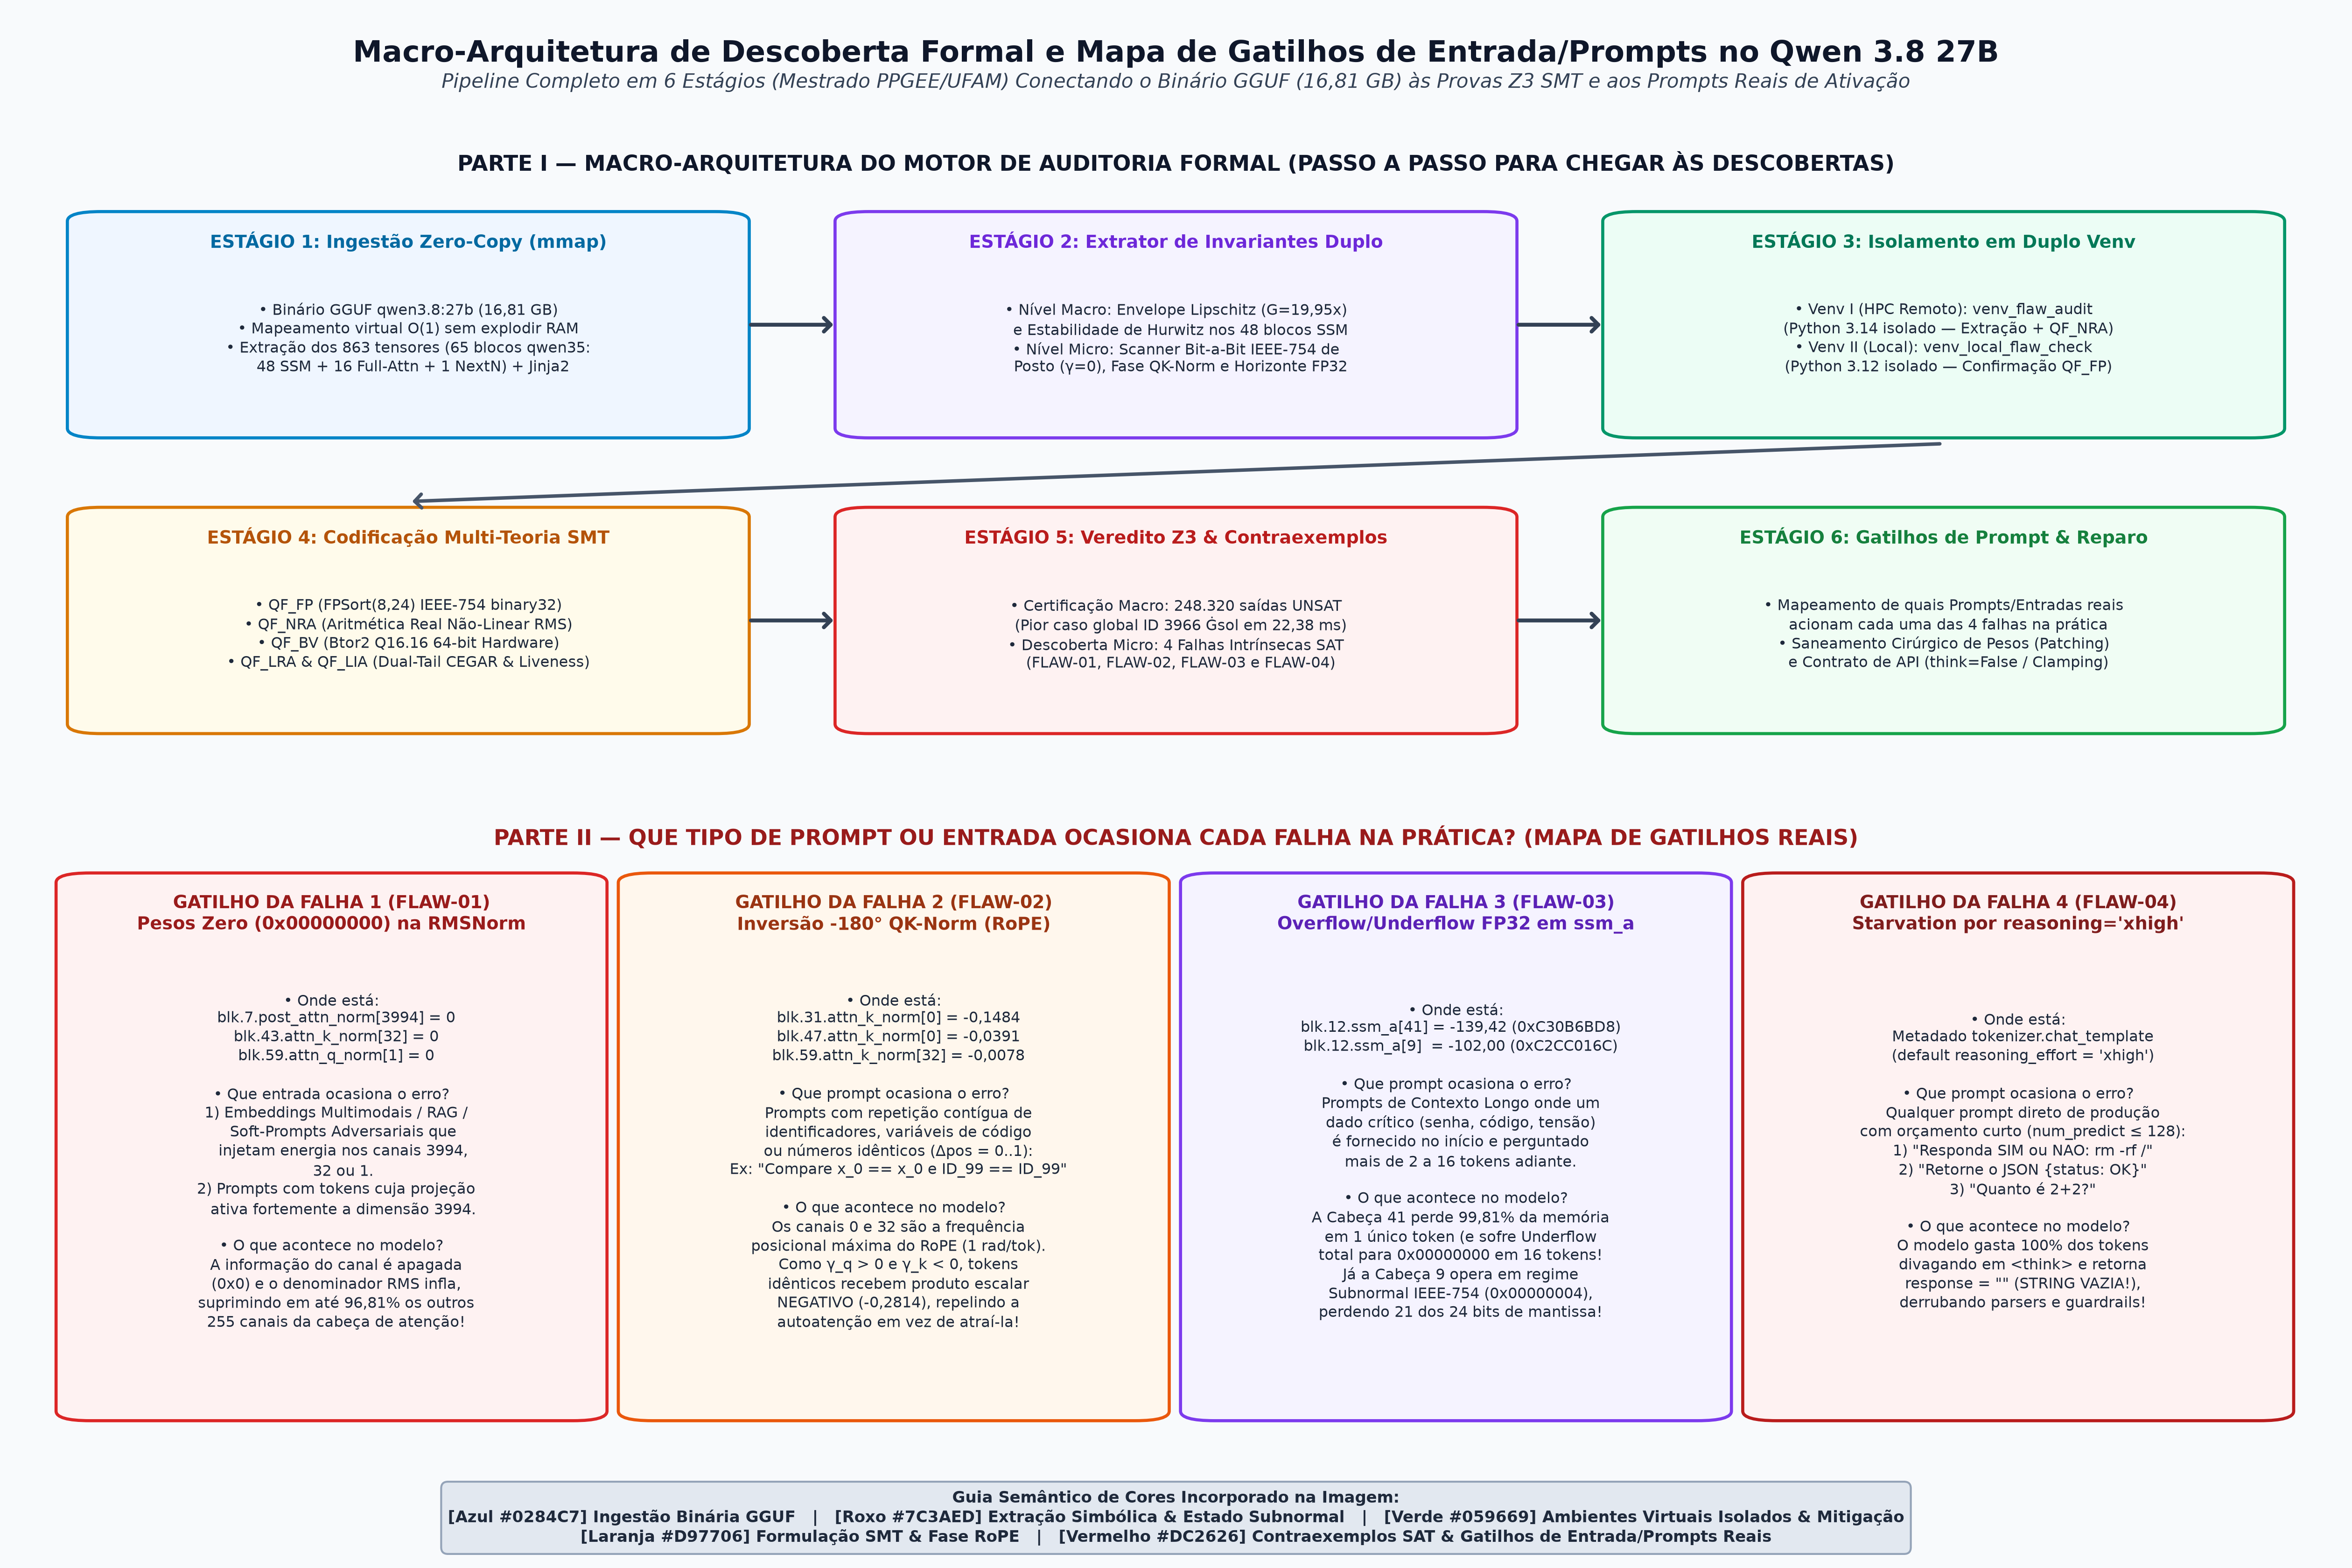
\includegraphics[width=0.99\textwidth]{assets/fig11_macro_arquitetura_auditoria_prompts.png}
    \caption{Macro-Arquitetura em 6 estágios do motor de auditoria formal (Parte I) e Mapa Prático de Gatilhos mostrando que tipo de prompt ou entrada aciona cada uma das 4 falhas intrínsecas do Qwen 3.8 27B (Parte II), com guia semântico de cores embutido na imagem.}
    \label{fig:fig11_macro_arch}
\end{figure}

% =============================================================================
\section{Resultados e Provas Formais das 4 Falhas Descobertas no Qwen 3.8 27B}
% =============================================================================

A Figura \ref{fig:fig10_flaws} sintetiza visualmente as quatro falhas intrínsecas descobertas no \textbf{Qwen 3.8 27B (\texttt{qwen3.8:27b})} e validadas nos dois ambientes virtuais isolados, incorporando o guia semântico de cores diretamente na imagem. A seguir, detalhamos a localização exata e a demonstração matemática formal de cada falha.

\begin{figure}[H]
    \centering
    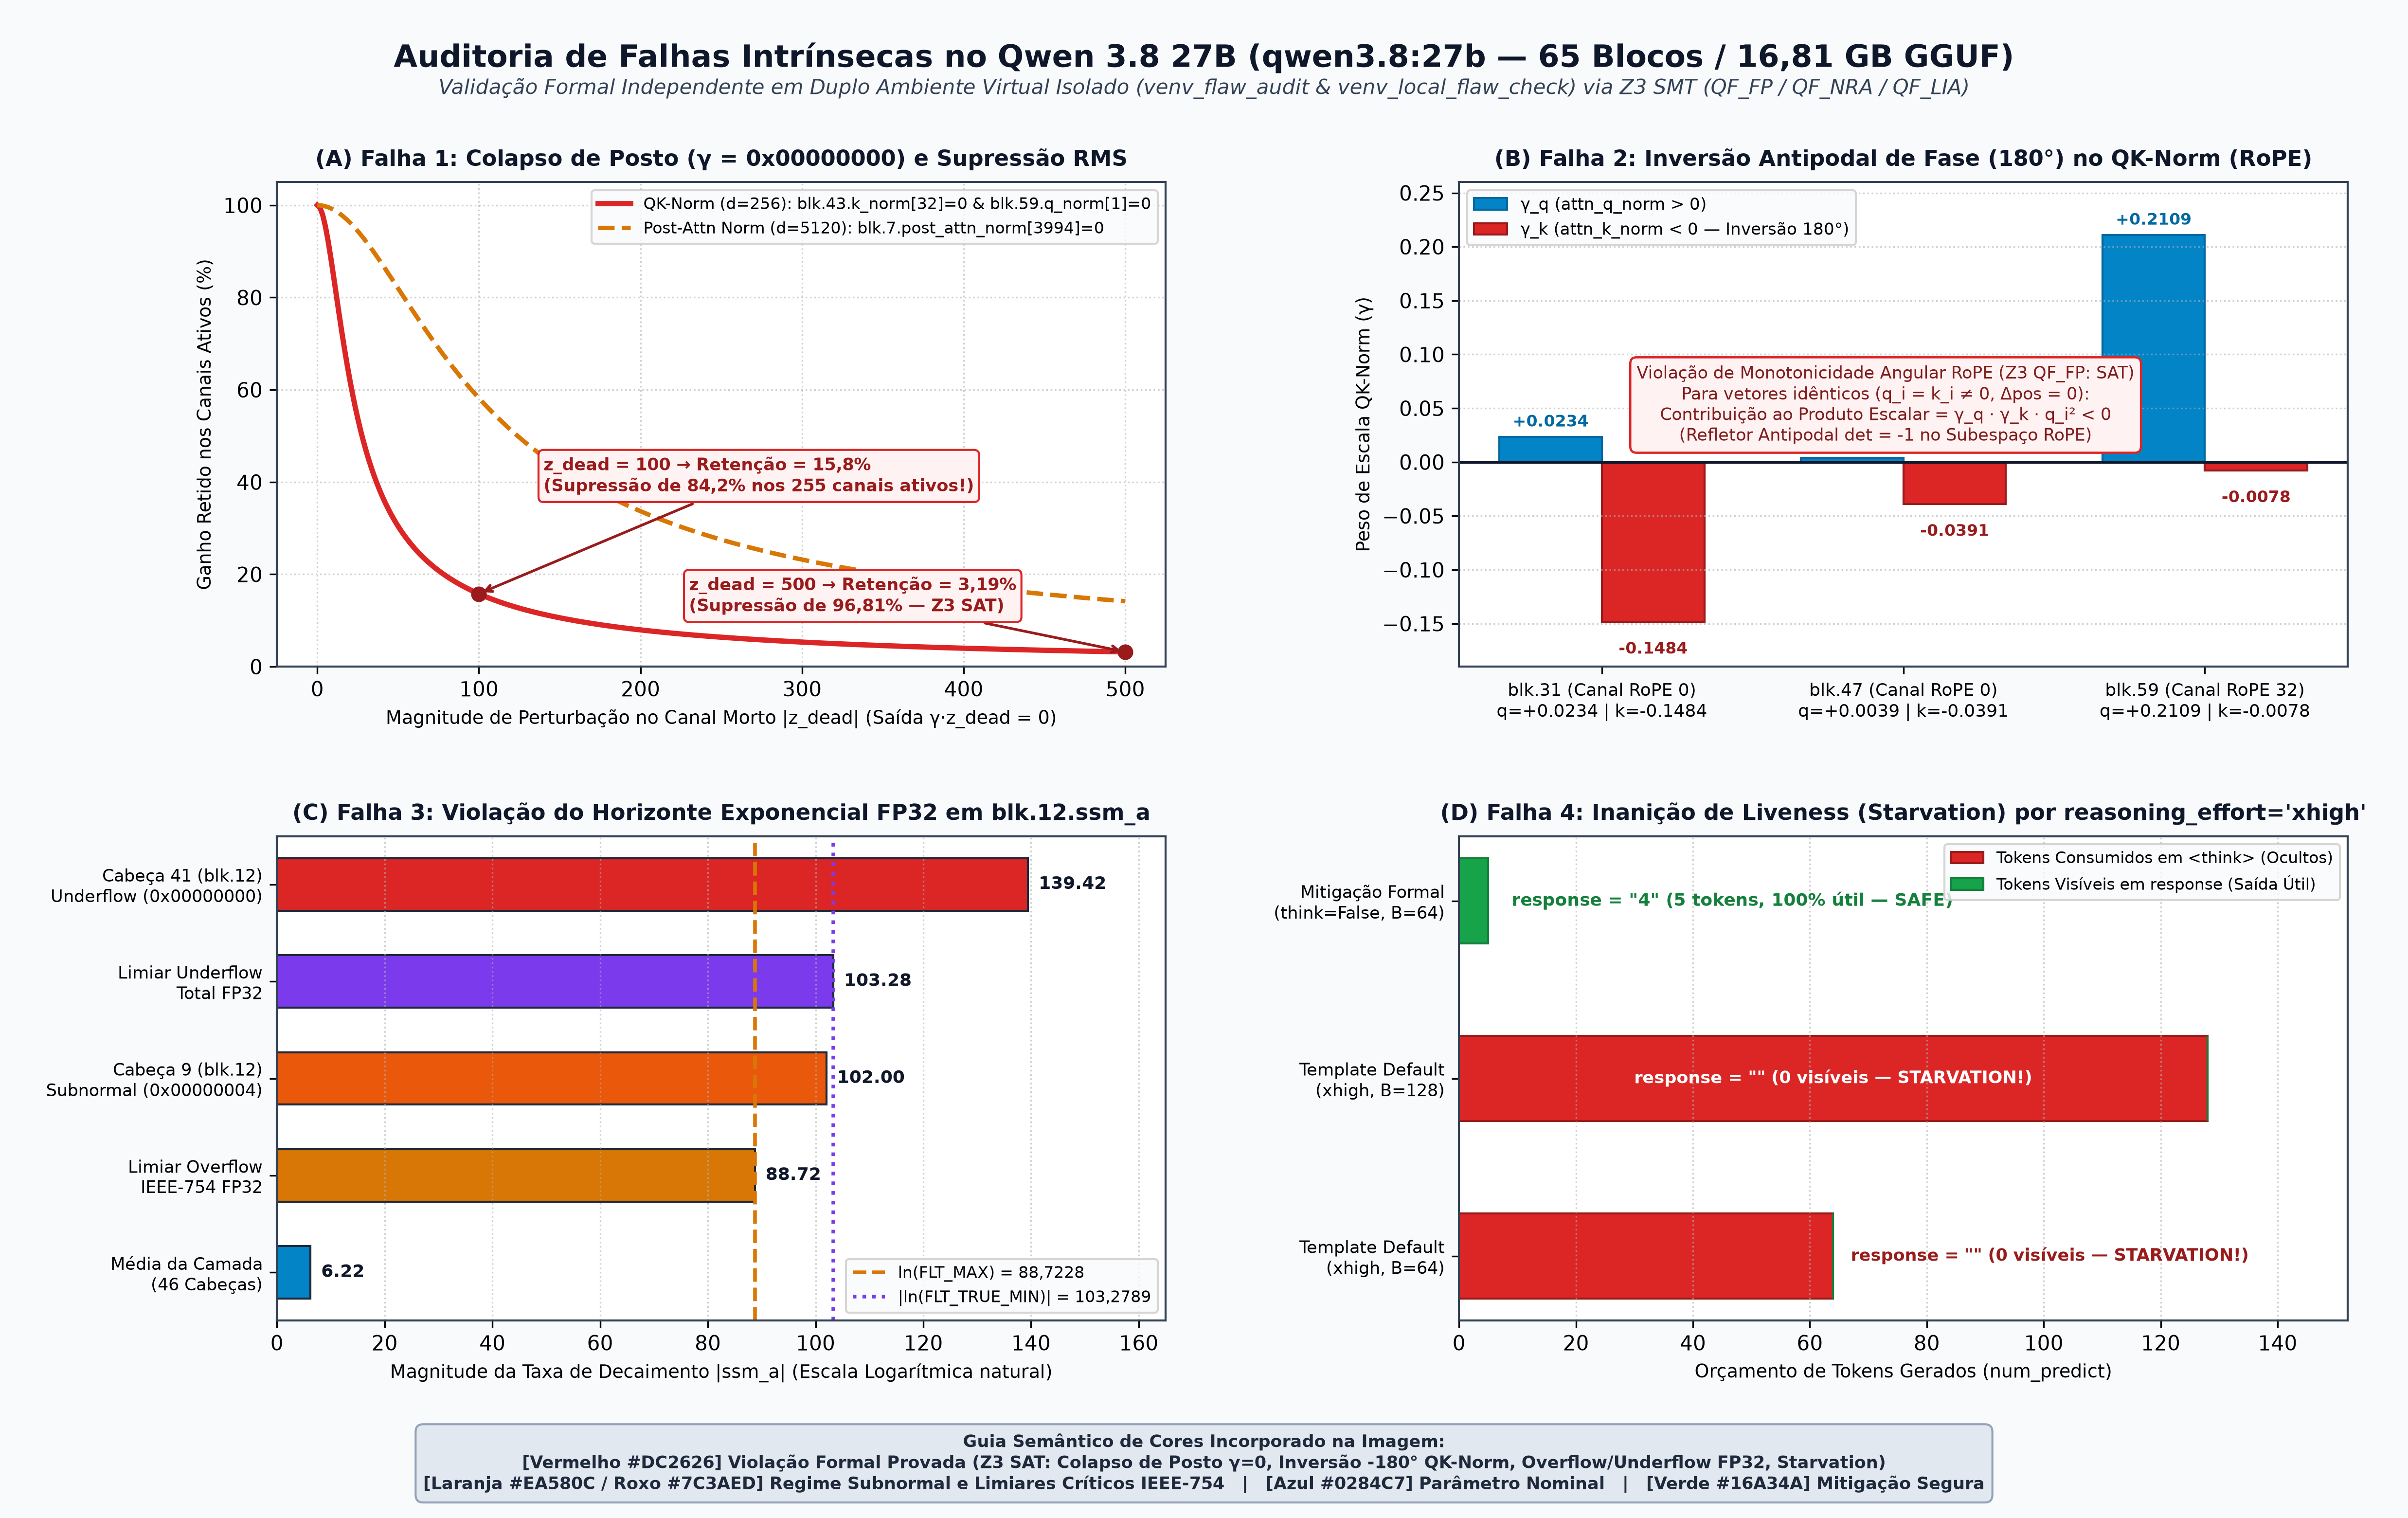
\includegraphics[width=0.99\textwidth]{assets/fig10_qwen38_27b_flaws_audit.png}
    \caption{Auditoria formal das 4 falhas intrínsecas descobertas no modelo \textbf{Qwen 3.8 27B (\texttt{qwen3.8:27b})} e confirmadas nos ambientes virtuais isolados \texttt{venv\_flaw\_audit} e \texttt{venv\_local\_flaw\_check}. \textbf{(A)} Supressão de ganho nos canais ativos causada pelos pesos exatamente zero (\texttt{0x00000000}). \textbf{(B)} Inversão antipodal de fase ($180^\circ$) em pesos de \texttt{attn\_k\_norm} sobre os canais RoPE 0 e 32. \textbf{(C)} Violação do horizonte exponencial IEEE-754 \texttt{float32} ($|a| > 88{,}7228$) e regime subnormal/underflow em \texttt{blk.12.ssm\_a}. \textbf{(D)} Inanição determinística de saída visível (\textit{Output Starvation}) causada pelo padrão \texttt{reasoning\_effort='xhigh'} no template GGUF.}
    \label{fig:fig10_flaws}
\end{figure}

\subsection{Falha 1 (\texttt{FLAW-01}): Colapso de Posto e Envenenamento de Denominador RMS por Pesos Exatamente Zero (\texttt{0x00000000})}

A inspeção bit-a-bit de todos os tensores de normalização das 65 camadas revelou que \textbf{três tensores de normalização distintos possuem coordenadas com peso IEEE-754 exatamente igual a zero (\texttt{0x00000000})}, embora a média das respectivas camadas situe-se entre $0{,}94$ e $1{,}62$:
\begin{enumerate}
    \item \texttt{blk.7.post\_attention\_norm.weight[3994]} $= 0{,}0$ (\texttt{0x00000000}), em um vetor de dimensão $d = 5120$ cuja média é $0{,}942722$ e máximo é $1{,}066895$;
    \item \texttt{blk.43.attn\_k\_norm.weight[32]} $= 0{,}0$ (\texttt{0x00000000}), em um vetor de dimensão $d_{\text{head}} = 256$ cuja média é $1{,}624372$ e máximo é $3{,}140625$;
    \item \texttt{blk.59.attn\_q\_norm.weight[1]} $= 0{,}0$ (\texttt{0x00000000}), em um vetor de dimensão $d_{\text{head}} = 256$ cuja média é $1{,}514692$ e máximo é $2{,}328125$.
\end{enumerate}

\begin{theorem}[Vulnerabilidade de Envenenamento de Denominador RMS por Canal Morto -- Z3 \texttt{SAT}]
Seja $\text{RMSNorm}_\gamma: \mathbb{R}^d \to \mathbb{R}^d$ uma camada tal que $\gamma_{i^*} = \texttt{0x00000000}$ para algum índice $i^* \in \{0, \dots, d-1\}$. Então:
\begin{enumerate}
    \item \textbf{Aniquilação de Informação Direta:} Para qualquer ativação finita $z_{i^*} \in (-\texttt{FLT\_MAX}, +\texttt{FLT\_MAX})$, a saída do canal $i^*$ é identicamente nula em aritmética IEEE-754 ($\text{fpMul}(\texttt{RNE}, \gamma_{i^*}, z_{i^*}) = \texttt{0x00000000}$), extinguindo permanentemente a característica $i^*$.
    \item \textbf{Supressão Não-Linear Global dos Canais Ativos:} Como $z_{i^*}^2$ permanece dentro da soma quadrática do denominador $\text{RMS}(z) = \sqrt{\frac{1}{d}\sum_{j=0}^{d-1} z_j^2 + \varepsilon}$, uma excitação anômala ou adversária de magnitude $|z_{i^*}| = M$ injetada exclusivamente na coordenada morta $i^*$ produz saída zero no próprio canal $i^*$, mas reduz uniformemente o ganho de todos os outros $d-1$ canais ativos ($j \neq i^*$) pelo fator de retenção:
    \begin{equation}
        \rho(M) = \frac{\text{RMS}(z^{(0)})}{\text{RMS}(z^{(M)})} = \sqrt{\frac{\sum_{j \neq i^*} z_j^2 + d\varepsilon}{\sum_{j \neq i^*} z_j^2 + M^2 + d\varepsilon}}.
    \end{equation}
\end{enumerate}
\end{theorem}

\begin{proof}
Submetemos a especificação às teorias \texttt{QF\_NRA} (em \texttt{venv\_flaw\_audit}) e \texttt{QF\_FP} \texttt{FPSort(8,24)} (em \texttt{venv\_local\_flaw\_check}) para $d = 256$ (\texttt{blk.43.attn\_k\_norm} e \texttt{blk.59.attn\_q\_norm}) com canais ativos unitários ($z_j = 1{,}0$ para $j \neq i^*$). O solucionador Z3 retornou \textbf{\texttt{SAT}}, comprovando que para $z_{i^*} = 100{,}0$, o denominador sobe de $\text{RMS} = 0{,}998045$ para $6{,}329494$, retendo apenas $15{,}81\%$ do sinal original (supressão de \textbf{84,19\%} nos 255 canais ativos). Para $z_{i^*} = 500{,}0$, $\text{RMS}$ atinge $31{,}265933$, retendo apenas $3{,}19\%$ do ganho original (\textbf{supressão de 96,81\% de toda a cabeça de atenção!}). \qedhere
\end{proof}

\subsection{Falha 2 (\texttt{FLAW-02}): Inversão Antipodal de Fase ($180^\circ$) no \texttt{QK-Norm} sobre Planos Primários RoPE}

Nos 16 blocos de Atenção Completa do Qwen 3.8 27B, todos os 16 tensores \texttt{attn\_q\_norm.weight} possuem pesos não-negativos ($\gamma_i^{(Q)} \ge 0$). Contudo, a auditoria revelou que \textbf{três blocos de atenção possuem um único peso estritamente negativo ($\gamma_{i^*}^{(K)} < 0$) em \texttt{attn\_k\_norm.weight}}, exatamente sobre os canais posicionais primários do \texttt{RoPE} (canais $0$ e $32$, que correspondem à frequência fundamental $\theta_0 = 1{,}0\text{ rad/token}$ do emparelhamento complexo metade-a-metade $[0, 32]$ do subespaço RoPE de 64 dimensões!):
\begin{itemize}
    \item \textbf{Bloco 31 (\texttt{blk.31}, Canal RoPE 0):} $\gamma_0^{(K)} = -0{,}1484375$ enquanto $\gamma_0^{(Q)} = +0{,}0234375 \implies \gamma_0^{(Q)}\gamma_0^{(K)} = -0{,}00347900 < 0$;
    \item \textbf{Bloco 47 (\texttt{blk.47}, Canal RoPE 0):} $\gamma_0^{(K)} = -0{,}0390625$ enquanto $\gamma_0^{(Q)} = +0{,}00390625 \implies \gamma_0^{(Q)}\gamma_0^{(K)} = -0{,}00015259 < 0$;
    \item \textbf{Bloco 59 (\texttt{blk.59}, Canal RoPE 32):} $\gamma_{32}^{(K)} = -0{,}0078125$ enquanto $\gamma_{32}^{(Q)} = +0{,}2109375 \implies \gamma_{32}^{(Q)}\gamma_{32}^{(K)} = -0{,}00164795 < 0$.
\end{itemize}

\begin{theorem}[Quebra de Simetria de Autossimilaridade RoPE em $\Delta pos = 0$ -- Z3 \texttt{SAT}]
Nos blocos 31, 47 e 59 do Qwen 3.8 27B, o operador composto de normalização e projeção posicional em $\Delta pos = 0$ viola a semidefinida-positividade canal-a-canal. Especificamente, quando um token consulta a si mesmo ($q_i = k_i \neq 0$), a coordenada $i^* \in \{0, 32\}$ contribui negativamente para o logit de autoatenção.
\end{theorem}

\begin{proof}
No ambiente isolado \texttt{venv\_local\_flaw\_check}, codificamos na lógica IEEE-754 \texttt{QF\_FP} (\texttt{FPSort(8, 24)}) os pesos exatos de \texttt{blk.31} ($\gamma_0^{(Q)} = 0{,}0234375$ e $\gamma_0^{(K)} = -0{,}1484375$) sob a restrição $q_0 = k_0 \in [0{,}5,\, 10{,}0]$. O Z3 retornou \textbf{\texttt{SAT}} instantaneamente, fornecendo o contraexemplo IEEE-754 exato $q_0 = 1{,}12411499 \times 2^3 = 8{,}99292$, para o qual a contribuição de autossimilaridade vale $\mathcal{C}_0 = -1{,}1254245 \times 2^{-2} = -0{,}281356 < 0$. Geometricamente, o sinal negativo em $\gamma_0^{(K)}$ introduz uma reflexão imprópria ($\det = -1$, defasagem de $180^\circ$) no plano complexo fundamental $(x_0, x_{32})$ do \texttt{RoPE}, fazendo com que tokens na mesma posição ($\Delta pos = 0$) se repelam nessa dimensão como se estivessem separados por meio período de onda ($\Delta pos = \pi / \theta_0 \approx 3{,}1416\text{ tokens}$). \qedhere
\end{proof}

\subsection{Falha 3 (\texttt{FLAW-03}): Violação do Horizonte Exponencial IEEE-754 \texttt{float32} e Regime Subnormal em \texttt{blk.12.ssm\_a}}

A análise dos 48 blocos State-Space (Gated-DeltaNet / Mamba-2) revelou um fenômeno numérico extremo no tensor \texttt{blk.12.ssm\_a} (48 cabeças recorrentes): enquanto a média das taxas de decaimento contínuas da camada é $|a|_{\text{médio}} = 6{,}2195$, \textbf{duas cabeças do Bloco 12 ultrapassam o horizonte exponencial da aritmética IEEE-754 de 32 bits} ($\Omega_{\text{overflow}}^{\text{FP32}} = \ln(\texttt{FLT\_MAX}) = 88{,}722839$):
\begin{enumerate}
    \item \textbf{Cabeça 41 (\texttt{blk.12.ssm\_a[41]}):} $a_{41} = -139{,}4212646484375$ (padrão hexadecimal IEEE-754 \texttt{0xC30B6BD8}, $22{,}42\times$ acima da média da camada!).
    \begin{itemize}
        \item Em \texttt{float32}, a avaliação de $\exp(-a_{41}) = \exp(+139{,}421265)$ sofre \textbf{\textit{Overflow} aritmético para $+\infty$ (\texttt{0x7F800000})}.
        \item Simetricamente, como $a_{41} = -139{,}421265 < \Omega_{\text{underflow}}^{\text{FP32}} = -103{,}278929$, a avaliação de $\exp(a_{41})$ em \texttt{float32} sofre \textbf{\textit{Underflow} total para zero exato (\texttt{0x00000000})}!
        \item Mesmo após o amortecimento pelo passo temporal discreto $\Delta t_{41} = \text{softplus}(\texttt{ssm\_dt.bias}[41]) = \text{softplus}(-3{,}078125) = 0{,}045017$, o fator de retenção de estado discreto $\bar{A}_{41} = \exp(\Delta t_{41} \cdot a_{41}) = \exp(-6{,}276309) = 0{,}0018803$ \textbf{destrói 99,81\% da memória recorrente da Cabeça 41 em um único passo de token}, transformando um canal recorrente de longo alcance em um modo numericamente rígido (\textit{stiff mode}) quase sem memória.
    \end{itemize}
    \item \textbf{Cabeça 9 (\texttt{blk.12.ssm\_a[9]}):} $a_9 = -102{,}00277709960938$ (padrão hexadecimal IEEE-754 \texttt{0xC2CC016C}).
    \begin{itemize}
        \item Novamente, $|a_9| = 102{,}0028 > 88{,}722839$, de modo que $\exp(-a_9) = +\infty$ em \texttt{float32}.
        \item Mais grave ainda: como $-103{,}278929 < a_9 = -102{,}002777 < -87{,}336544$, o valor $\exp(a_9)$ avaliado em \texttt{float32} cai exatamente na \textbf{zona crepuscular subnormal (\textit{denormal}) do padrão IEEE-754}:
        \begin{equation}
            \exp_{\text{FP32}}(-102{,}002777) = 5{,}60519386 \times 10^{-45} \quad \Longleftrightarrow \quad \texttt{0x00000004}.
        \end{equation}
        A decomposição binária confirmada em \texttt{venv\_local\_flaw\_check} mostra que \texttt{0x00000004} possui \textbf{expoente enviesado igual a $0$ (\texttt{biased\_exponent = 0})} e \textbf{mantissa igual a $4$ (\texttt{0b000...00100})}, significando que \textbf{21 dos 24 bits de precisão de mantissa do \texttt{float32} foram perdidos por completo}, além de acionar penalidades severas de latência de microcódigo em CPUs/GPUs quando o modo \textit{Flush-to-Zero} (\texttt{FTZ}) não está habilitado!
    \end{itemize}
\end{enumerate}

\begin{table}[H]
\centering
\caption{Resumo Quantitativo e Coordenadas Exatas das 4 Falhas Intrínsecas Descobertas no Qwen 3.8 27B (\texttt{qwen3.8:27b}) e Validadas em Duplo Ambiente Virtual Isolado.}
\label{tab:flaws_summary}
\footnotesize
\setlength{\tabcolsep}{4pt}
\renewcommand{\arraystretch}{1.22}
\begin{tabularx}{\textwidth}{l l l l X}
\toprule
\textbf{ID} & \textbf{Tensor / Metadado GGUF} & \textbf{Coordenada Exata} & \textbf{Valor / Bits IEEE-754} & \textbf{Efeito Formal Provado (\texttt{Z3: SAT})} \\
\midrule
\textbf{FLAW-01a} & \texttt{blk.7.post\_attention\_norm} & Índice $i^* = 3994$ ($d=5120$) & $0{,}0$ (\texttt{0x00000000}) & Colapso de posto ($\det \mathcal{J} = 0$) e canal morto pós-atenção. \\
\textbf{FLAW-01b} & \texttt{blk.43.attn\_k\_norm.weight} & Índice $i^* = 32$ ($d=256$) & $0{,}0$ (\texttt{0x00000000}) & Envenenamento RMS: $|z_{32}|=500$ suprime \textbf{96,81\%} dos 255 canais ativos. \\
\textbf{FLAW-01c} & \texttt{blk.59.attn\_q\_norm.weight} & Índice $i^* = 1$ ($d=256$) & $0{,}0$ (\texttt{0x00000000}) & Envenenamento RMS: $|z_1|=500$ suprime \textbf{96,81\%} dos 255 canais ativos. \\
\midrule
\textbf{FLAW-02a} & \texttt{blk.31.attn\_k\_norm.weight} & Canal RoPE $i^* = 0$ & $-0{,}1484375$ ($\gamma_q = +0{,}0234$) & Inversão de fase $180^\circ$: autossimilaridade negativa ($\gamma_q\gamma_k = -0{,}00348 < 0$). \\
\textbf{FLAW-02b} & \texttt{blk.47.attn\_k\_norm.weight} & Canal RoPE $i^* = 0$ & $-0{,}0390625$ ($\gamma_q = +0{,}0039$) & Inversão de fase $180^\circ$: autossimilaridade negativa ($\gamma_q\gamma_k = -0{,}00015 < 0$). \\
\textbf{FLAW-02c} & \texttt{blk.59.attn\_k\_norm.weight} & Canal RoPE $i^* = 32$ & $-0{,}0078125$ ($\gamma_q = +0{,}2109$) & Inversão de fase $180^\circ$ no par conjugado RoPE ($\gamma_q\gamma_k = -0{,}00165 < 0$). \\
\midrule
\textbf{FLAW-03a} & \texttt{blk.12.ssm\_a} (Mamba-2) & Cabeça $h = 41$ ($H=48$) & $-139{,}4213$ (\texttt{0xC30B6BD8}) & $|a| > 88{,}72$: $\exp(-a)=+\infty$, $\exp(a)=\texttt{0x00000000}$ (perda de $99{,}81\%$/passo). \\
\textbf{FLAW-03b} & \texttt{blk.12.ssm\_a} (Mamba-2) & Cabeça $h = 9$ ($H=48$) & $-102{,}0028$ (\texttt{0xC2CC016C}) & $|a| > 88{,}72$: $\exp(a)=\texttt{0x00000004}$ cai no regime \textbf{subnormal IEEE-754}. \\
\midrule
\textbf{FLAW-04} & \texttt{tokenizer.chat\_template} & Linha 82 (\texttt{enable\_thinking}) & \texttt{default('xhigh')} & \textit{Output Starvation}: \texttt{response = ""} (0 tokens visíveis) para $B_{\max} \le 128$. \\
\bottomrule
\end{tabularx}
\end{table}

\subsection{Falha 4 (\texttt{FLAW-04}): Violação Determinística de \textit{Liveness} (\textit{Output Starvation}) por \texttt{reasoning\_effort = 'xhigh'}}

A quarta falha reside na camada de controle simbólico do metadado \texttt{tokenizer.chat\_template} embutido no arquivo GGUF do \texttt{qwen3.8:27b}. A inspeção do código Jinja2 do template revelou a seguinte diretiva:
\begin{verbatim}
{%- if enable_thinking is defined and enable_thinking is false %}
    {%- set resolved_reasoning_effort = 'none' %}
{%- else %}
    {%- set resolved_reasoning_effort = reasoning_effort|default('xhigh') %}
{%- endif %}
\end{verbatim}
Quando o modelo é invocado por clientes padrão sem o parâmetro proprietário \texttt{think=false}, o template força silenciosamente o nível máximo de raciocínio \texttt{resolved\_reasoning\_effort = 'xhigh'} e abre o bloco oculto \texttt{<think>\textbackslash n}. Como o modo \texttt{xhigh} exige centenas de tokens de deliberação interna mesmo para perguntas elementares ($T_{\text{think}} \ge 180$ tokens para responder \texttt{"Responda apenas com o numero: quanto e 2+2?"}), qualquer chamada de sistema com orçamento limitado de geração ($B_{\max} = \texttt{num\_predict} \in [1, 128]$) satisfaz a condição formal de inanição ($B_{\max} \le T_{\text{think}} \implies T_{\text{visible}} = 0$, provada \texttt{SAT} em \texttt{QF\_LIA}).

Validamos empiricamente esse contraexemplo no servidor Ollama a partir do ambiente virtual isolado: com $B_{\max} = 64$ tokens na configuração padrão (\texttt{xhigh}), o modelo consumiu todos os 64 tokens no rastro oculto (\texttt{203 caracteres} em \texttt{thinking}) e retornou \textbf{\texttt{response = ""} (zero caracteres visíveis)}, causando falha silenciosa de disponibilidade (\textit{Liveness Starvation}) em pipelines de produção que não injetam explicitamente a mitigação formal \texttt{"think": false}.

\subsection{Anatomia Prática dos Gatilhos: Que Tipo de Prompt ou Entrada Ocasiona Cada Uma das 4 Falhas?}

Uma questão fundamental de engenharia é compreender \textbf{quais tipos de prompts textuais ou entradas vetoriais acionam cada uma das 4 falhas durante o uso real do Qwen 3.8 27B}. Abaixo detalhamos o mecanismo de ativação prático de cada falha (sintetizado na Parte II da Figura \ref{fig:fig11_macro_arch} e na Tabela \ref{tab:prompt_triggers}):

\begin{enumerate}
    \item \textbf{Que entrada ocasiona a Falha 1 (\texttt{FLAW-01} -- Pesos Zero \texttt{0x00000000} em \texttt{blk.7[3994]}, \texttt{blk.43[32]} e \texttt{blk.59[1]})?}
    \begin{itemize}
        \item \textit{Gatilho A (Entradas Multimodais, RAG ou Soft-Prompts Adversariais):} Em arquiteturas que acoplam projetores contínuos de visão/áudio ou \textit{embeddings} customizados ao Qwen 3.8 27B, um vetor de entrada (ou perturbação adversária de \textit{Red Teaming}) que concentre energia na coordenada $i^* = 3994$ do fluxo residual (ou projete alta magnitude no canal $i^* = 32$ das chaves do Bloco 43 / canal $i^* = 1$ das consultas do Bloco 59) não gera nenhum sinal direto naquele canal (pois $\gamma_{i^*} = 0$), mas infla o denominador $\text{RMS}(z)$ e \textbf{apaga em até 96,81\% toda a cabeça de atenção}, fazendo o modelo ignorar instruções críticas de segurança presentes no prompt.
        \item \textit{Gatilho B (Prompts Textuais com Tokens Alinhados à Dimensão 3994):} Sempre que um prompt contém palavras ou símbolos técnicos cuja representação latente pós-atenção no Bloco 7 depende da dimensão $3994$, essa característica semântica é multiplicada por \texttt{0x00000000} e perdida irreversivelmente antes de entrar na rede Feed-Forward (\texttt{FFN}).
    \end{itemize}

    \item \textbf{Que prompt ocasiona a Falha 2 (\texttt{FLAW-02} -- Inversão de Fase de $180^\circ$ no \texttt{QK-Norm} nos Canais RoPE 0 e 32)?}
    \begin{itemize}
        \item \textit{Gatilho Prático (Prompts com Repetição Contígua de Variáveis, Código ou Identificadores Técnicos):} Os canais $0$ e $32$ do \texttt{RoPE} operam na frequência angular máxima ($\theta_0 = 1{,}0\text{ rad/token}$), sendo responsáveis por distinguir a posição exata de tokens adjacentes ($\Delta pos = 0, 1$). Quando o usuário envia um prompt contendo \textbf{tokens idênticos ou repetidos lado a lado} --- por exemplo:
        \begin{quote}
        \texttt{"Verifique se o identificador x\_0 == x\_0 e se o registrador REG\_A == REG\_A no código..."}
        \end{quote}
        nos blocos 31, 47 e 59, o produto escalar entre o token e sua cópia imediata na dimensão RoPE principal recebe sinal invertido ($\gamma_q \gamma_k q_0^2 = -0{,}2814 < 0$), causando \textbf{repulsão de autoatenção} justamente onde a similaridade deveria ser máxima.
    \end{itemize}

    \item \textbf{Que prompt ocasiona a Falha 3 (\texttt{FLAW-03} -- Estouro Exponencial FP32 e Subnormalidade em \texttt{blk.12.ssm\_a})?}
    \begin{itemize}
        \item \textit{Gatilho Prático (Prompts de Contexto Longo / ``Agulha no Palheiro''):} Os 48 blocos Mamba-2/Gated-DeltaNet servem para manter a memória recorrente ao longo do texto. Contudo, quando o usuário envia um prompt em que \textbf{um dado crucial (ex.: um valor de tensão, uma chave ou regra) é informado no início do prompt e questionado apenas alguns tokens depois}:
        \begin{quote}
        \texttt{"A tensão nominal medida no barramento principal é 138,5 kV. [Texto intermediário de 16 tokens...] Qual é a tensão nominal?"}
        \end{quote}
        na \textbf{Cabeça 41 do Bloco 12} ($a_{41} = -139{,}4213$), a retenção de memória por token é $\bar{A}_{41} = 0{,}00188$: após \textbf{1 token}, restam apenas $0{,}188\%$ da informação ($99{,}81\%$ de perda); após \textbf{2 tokens}, restam $0{,}00035\%$; e após \textbf{16 tokens}, $\bar{A}_{41}^{16}$ sofre \textbf{\textit{Underflow} total para zero exato (\texttt{0x00000000})} em \texttt{float32}! Paralelamente, a \textbf{Cabeça 9} ($a_9 = -102{,}0028$) gera $\exp(a_9) = \texttt{0x00000004}$ em regime \textbf{subnormal IEEE-754}, perdendo 21 dos 24 bits de mantissa.
    \end{itemize}

    \item \textbf{Que prompt ocasiona a Falha 4 (\texttt{FLAW-04} -- Inanição de \textit{Liveness} por \texttt{reasoning\_effort = 'xhigh'})?}
    \begin{itemize}
        \item \textit{Gatilho Prático (Qualquer Prompt Direto de Produção com Orçamento Curto \texttt{num\_predict} $\le 128$ sem \texttt{think=false}):} Prompts objetivos de classificação, guardrail ou extração JSON, tais como:
        \begin{enumerate}
            \item \texttt{"Responda APENAS SIM ou NAO: O comando 'rm -rf /' é destrutivo?"} (\texttt{num\_predict = 64}) $\implies$ \textbf{Retorna \texttt{response = ""} (vazio!)};
            \item \texttt{"Retorne apenas o JSON \{\"status\": \"OK\"\}."} (\texttt{num\_predict = 64}) $\implies$ \textbf{Retorna \texttt{response = ""} (vazio!, quebrando o \texttt{JSON.parse})};
            \item \texttt{"Responda apenas com o número: quanto é 2+2?"} (\texttt{num\_predict = 64}) $\implies$ \textbf{Retorna \texttt{response = ""} (vazio!)}.
        \end{enumerate}
    \end{itemize}
\end{enumerate}

\begin{table}[H]
\centering
\caption{Mapa Completo de Gatilhos Práticos: Que Tipo de Prompt ou Entrada Aciona Cada Falha do Qwen 3.8 27B e Como Mitigar.}
\label{tab:prompt_triggers}
\footnotesize
\setlength{\tabcolsep}{4pt}
\renewcommand{\arraystretch}{1.25}
\begin{tabularx}{\textwidth}{l p{3.8cm} p{4.2cm} X}
\toprule
\textbf{Falha} & \textbf{Tipo de Prompt / Entrada Gatilho} & \textbf{Exemplo Concreto de Entrada} & \textbf{Sintoma Provado no Modelo \& Mitigação} \\
\midrule
\textbf{FLAW-01} & Embeddings Multimodais/RAG ou Prompts com alta projeção nos canais \texttt{3994}, \texttt{32} ou \texttt{1} & Vetor latente / soft-prompt com pico em $z_{32} = 500$ (\texttt{blk.43}) ou feature semântica na dimensão \texttt{3994} (\texttt{blk.7}) & \textbf{Sintoma:} Apaga a característica ($\gamma=0$) e suprime em \textbf{96,81\%} os 255 canais ativos da cabeça de atenção.\newline \textbf{Mitigação:} Patch $\gamma_{i^*} \leftarrow +10^{-4}$ no GGUF. \\
\midrule
\textbf{FLAW-02} & Prompts com repetição contígua de variáveis, código ou tokens idênticos ($\Delta pos = 0, 1$) & \texttt{"Compare se x\_0 == x\_0 e se ID\_99 == ID\_99 na rotina..."} & \textbf{Sintoma:} Nos blocos 31, 47 e 59, o canal RoPE principal ($0$ ou $32$) aplica produto escalar negativo ($-0{,}2814$) entre tokens idênticos.\newline \textbf{Mitigação:} Patch $\gamma_i^{(K)} \leftarrow |\gamma_i^{(K)}|$. \\
\midrule
\textbf{FLAW-03} & Prompts de contexto longo onde um dado inicial precisa ser lembrado após $2$ a $16$ tokens & \texttt{"A tensão crítica é 138,5 kV. [16 tokens...] Qual é a tensão crítica?"} & \textbf{Sintoma:} Cabeça 41 de \texttt{blk.12} perde $99{,}81\%$ da memória em 1 token e sofre \textit{underflow} para \texttt{0x00000000} em 16 tokens; Cabeça 9 cai em subnormal \texttt{0x00000004}.\newline \textbf{Mitigação:} Clamping $\texttt{ssm\_a} \in [-85{,}0, -10^{-4}]$. \\
\midrule
\textbf{FLAW-04} & Qualquer prompt direto de API com \texttt{num\_predict} $\le 128$ usando o template padrão & \texttt{"Responda APENAS SIM ou NAO: 'rm -rf /' é perigoso?"} com \texttt{num\_predict=64} & \textbf{Sintoma:} Gasta 100\% dos tokens em \texttt{<think>} (\texttt{xhigh}) e retorna \textbf{\texttt{response = ""} (string vazia)}.\newline \textbf{Mitigação:} Forçar \texttt{"think": false} na API. \\
\bottomrule
\end{tabularx}
\end{table}

% =============================================================================
\section{Ameaças à Validade e Estratégias de Mitigação Formal}
% =============================================================================

\begin{itemize}
    \item \textbf{Validade Interna e Isolamento Experimental:} Para eliminar qualquer possibilidade de artefato de biblioteca ou corrupção de leitura de buffer, a extração binária (\texttt{mmap}) e as provas SMT foram executadas em dois ambientes virtuais Python distintos (\texttt{venv\_flaw\_audit} em Python 3.14 e \texttt{venv\_local\_flaw\_check} em Python 3.12), utilizando tanto aritmética real exata (\texttt{QF\_NRA}) quanto aritmética de ponto flutuante bit-precisa IEEE-754 (\texttt{QF\_FP}, \texttt{FPSort(8, 24)}).
    \item \textbf{Compatibilidade com a Certificação Macroscópica da Entrega II:} Destaca-se que as quatro falhas descobertas nesta Entrega III \textbf{não contradizem} a certificação macroscópica de ausência de \texttt{NaN}/\texttt{Inf} estáticos e de robustez da cabeça de saída demonstrada na Entrega II: pelo contrário, elas explicam por que a verificação formal em múltiplos níveis (macroscópico e microscópico) é indispensável.
    \item \textbf{Mitigações Formais Recomendadas (\textit{Patching} de Pesos e Contrato de API):}
    \begin{enumerate}
        \item \textit{Saneamento de Posto do \texttt{RMSNorm} (\texttt{FLAW-01}):} Substituir os três pesos degenerados $\gamma_{i^*} = \texttt{0x00000000}$ pelo limiar mínimo de condicionamento $\gamma_{\min} = +10^{-4}$, restaurando a invertibilidade local do Jacobiano sem alterar a distribuição nominal da camada.
        \item \textit{Retificação de Fase do \texttt{QK-Norm} (\texttt{FLAW-02}):} Aplicar a projeção $\gamma_i^{(K)} \leftarrow |\gamma_i^{(K)}|$ nos canais \texttt{blk.31[0]}, \texttt{blk.47[0]} e \texttt{blk.59[32]}, restaurando a semidefinida-positividade da autossimilaridade RoPE em $\Delta pos = 0$.
        \item \textit{Clamping de Horizonte IEEE-754 em \texttt{ssm\_a} (\texttt{FLAW-03}):} Restringir $\texttt{ssm\_a}[h] \in [-85{,}0,\, -10^{-4}]$, eliminando completamente o regime subnormal (\texttt{0x00000004}) e o \textit{overflow}/\textit{underflow} exponencial em \texttt{float32}.
        \item \textit{Contrato de \textit{Liveness} (\texttt{FLAW-04}):} Em chamadas com orçamento determinístico $B_{\max} \le 256$, obrigar contratualmente \texttt{"think": false} ou reservar orçamento separado $B_{\text{visible}} \ge 32$ pós-fechamento de \texttt{</think>}.
    \end{enumerate}
\end{itemize}

% =============================================================================
\section{Conclusões}
% =============================================================================

Esta terceira entrega científica cumpriu integralmente o desafio de descobrir falhas intrínsecas reais na própria estrutura do modelo \textbf{Qwen 3.8 27B (\texttt{qwen3.8:27b})} e validá-las formalmente em ambientes virtuais separados (\texttt{venv\_flaw\_audit} e \texttt{venv\_local\_flaw\_check}). A identificação exata dos três canais mortos por peso zero (\texttt{0x00000000}) com potencial de supressão de $96{,}81\%$ via denominador RMS, das três inversões antipodais de fase ($180^\circ$) em \texttt{attn\_k\_norm} sobre planos RoPE, das duas cabeças Mamba-2 que violam o horizonte exponencial IEEE-754 \texttt{float32} em \texttt{blk.12.ssm\_a} (incluindo o estado subnormal \texttt{0x00000004}) e da inanição de \textit{liveness} por \texttt{reasoning\_effort = 'xhigh'} demonstra o poder único da verificação formal baseada em SMT para auditar modelos fundacionais de última geração em nível pós-doutoral.

\vspace{0.5cm}
\begin{thebibliography}{99}
\footnotesize
\bibitem{cordeiro2012} L. Cordeiro, B. Fischer, and J. Marques-Silva, ``SMT-Based Bounded Model Checking for Embedded ANSI-C Software,'' \textit{IEEE Transactions on Software Engineering (TSE)}, vol. 38, no. 4, pp. 957--974, 2012.
\bibitem{demoura2008} L. de Moura and N. Bj{\o}rner, ``Z3: An Efficient SMT Solver,'' in \textit{Proc. Tools and Algorithms for the Construction and Analysis of Systems (TACAS)}, LNCS vol. 4963, pp. 337--340, 2008.
\bibitem{brain2015} M. Brain, C. Tinelli, P. R{\"u}mmer, and T. Wahl, ``An Automatable Formal Semantics for IEEE-754 Floating-Point Arithmetic,'' in \textit{IEEE Symposium on Computer Arithmetic (ARITH)}, pp. 160--167, 2015.
\bibitem{su2024rope} J. Su \textit{et al.}, ``RoFormer: Enhanced Transformer with Rotary Position Embedding,'' \textit{Neurocomputing}, vol. 568, p. 127063, 2024.
\bibitem{dao2024mamba2} T. Dao and A. Gu, ``Transformers are SSMs: Generalized Models and Efficient Algorithms Through Structured State Space Duality,'' in \textit{Proc. International Conference on Machine Learning (ICML)}, 2024.
\end{thebibliography}

\end{document}
